% !Mode:: "TeX:UTF-8"
\documentclass[12pt,a4paper]{article}

%%%%%%%%------------------------------------------------------------------------
%%%% 日常所用宏包

%% 控制页边距
% 如果是beamer文档类, 则不用geometry
\makeatletter
\@ifclassloaded{beamer}{}{\usepackage[top=2.5cm, bottom=2.5cm, left=2.5cm, right=2.5cm]{geometry}}
\makeatother

%% 控制项目列表
\usepackage{enumerate}

%% 多栏显示
\usepackage{multicol}

%% 算法环境
\usepackage{algorithm}  
\usepackage{algorithmic} 
\usepackage{float} 

%% 网址引用
\usepackage{url}

%% 控制矩阵行距
\renewcommand\arraystretch{1.4}

%% hyperref宏包,生成可定位点击的超链接,并且会生成pdf书签
\makeatletter
\@ifclassloaded{beamer}{
\usepackage{hyperref}
\usepackage{ragged2e} % 对齐
}{
\usepackage[%
    pdfstartview=FitH,%
    CJKbookmarks=true,%
    bookmarks=true,%
    bookmarksnumbered=true,%
    bookmarksopen=true,%
    colorlinks=true,%
    citecolor=blue,%
    linkcolor=blue,%
    anchorcolor=green,%
    urlcolor=blue%
]{hyperref}
}
\makeatother



\makeatletter % 如果是 beamer 不需要下面两个包
\@ifclassloaded{beamer}{
\mode<presentation>
{
} 
}{
%% 控制标题
\usepackage{titlesec}
%% 控制目录
\usepackage{titletoc}
}
\makeatother

%% 控制表格样式
\usepackage{booktabs}

%% 控制字体大小
\usepackage{type1cm}

%% 首行缩进,用\noindent取消某段缩进
\usepackage{indentfirst}

%% 支持彩色文本、底色、文本框等
\usepackage{color,xcolor}

%% AMS LaTeX宏包: http://zzg34b.w3.c361.com/package/maths.htm#amssymb
\usepackage{amsmath,amssymb}
%% 多个图形并排
\usepackage{subfig}
%%%% 基本插图方法
%% 图形宏包
\usepackage{graphicx}
\newcommand{\red}[1]{\textcolor{red}{#1}}
\newcommand{\blue}[1]{\structure{#1}}
\newcommand{\brown}[1]{\textcolor{brown}{#1}}
\newcommand{\green}[1]{\textcolor{green}{#1}}


%%%% 基本插图方法结束

%%%% pgf/tikz绘图宏包设置
\usepackage{pgf,tikz}
\usetikzlibrary{shapes,automata,snakes,backgrounds,arrows}
\usetikzlibrary{mindmap}
%% 可以直接在latex文档中使用graphviz/dot语言,
%% 也可以用dot2tex工具将dot文件转换成tex文件再include进来
%% \usepackage[shell,pgf,outputdir={docgraphs/}]{dot2texi}
%%%% pgf/tikz设置结束


\makeatletter % 如果是 beamer 不需要下面两个包
\@ifclassloaded{beamer}{

}{
%%%% fancyhdr设置页眉页脚
%% 页眉页脚宏包
\usepackage{fancyhdr}
%% 页眉页脚风格
\pagestyle{plain}
}

%% 有时会出现\headheight too small的warning
\setlength{\headheight}{15pt}

%% 清空当前页眉页脚的默认设置
%\fancyhf{}
%%%% fancyhdr设置结束


\makeatletter % 对 beamer 要重新设置
\@ifclassloaded{beamer}{

}{
%%%% 设置listings宏包用来粘贴源代码
%% 方便粘贴源代码,部分代码高亮功能
\usepackage{listings}

%% 设置listings宏包的一些全局样式
%% 参考http://hi.baidu.com/shawpinlee/blog/item/9ec431cbae28e41cbe09e6e4.html
\lstset{
showstringspaces=false,              %% 设定是否显示代码之间的空格符号
numbers=left,                        %% 在左边显示行号
numberstyle=\tiny,                   %% 设定行号字体的大小
basicstyle=\footnotesize,                    %% 设定字体大小\tiny, \small, \Large等等
keywordstyle=\color{blue!70}, commentstyle=\color{red!50!green!50!blue!50},
                                     %% 关键字高亮
frame=shadowbox,                     %% 给代码加框
rulesepcolor=\color{red!20!green!20!blue!20},
escapechar=`,                        %% 中文逃逸字符,用于中英混排
xleftmargin=2em,xrightmargin=2em, aboveskip=1em,
breaklines,                          %% 这条命令可以让LaTeX自动将长的代码行换行排版
extendedchars=false                  %% 这一条命令可以解决代码跨页时,章节标题,页眉等汉字不显示的问题
}}
\makeatother
%%%% listings宏包设置结束


%%%% 附录设置
\makeatletter % 对 beamer 要重新设置
\@ifclassloaded{beamer}{

}{
\usepackage[title,titletoc,header]{appendix}
}
\makeatother
%%%% 附录设置结束


%%%% 日常宏包设置结束
%%%%%%%%------------------------------------------------------------------------


%%%%%%%%------------------------------------------------------------------------
%%%% 英文字体设置结束
%% 这里可以加入自己的英文字体设置
%%%%%%%%------------------------------------------------------------------------

%%%%%%%%------------------------------------------------------------------------
%%%% 设置常用字体字号,与MS Word相对应

%% 一号, 1.4倍行距
\newcommand{\yihao}{\fontsize{26pt}{36pt}\selectfont}
%% 二号, 1.25倍行距
\newcommand{\erhao}{\fontsize{22pt}{28pt}\selectfont}
%% 小二, 单倍行距
\newcommand{\xiaoer}{\fontsize{18pt}{18pt}\selectfont}
%% 三号, 1.5倍行距
\newcommand{\sanhao}{\fontsize{16pt}{24pt}\selectfont}
%% 小三, 1.5倍行距
\newcommand{\xiaosan}{\fontsize{15pt}{22pt}\selectfont}
%% 四号, 1.5倍行距
\newcommand{\sihao}{\fontsize{14pt}{21pt}\selectfont}
%% 半四, 1.5倍行距
\newcommand{\bansi}{\fontsize{13pt}{19.5pt}\selectfont}
%% 小四, 1.5倍行距
\newcommand{\xiaosi}{\fontsize{12pt}{18pt}\selectfont}
%% 大五, 单倍行距
\newcommand{\dawu}{\fontsize{11pt}{11pt}\selectfont}
%% 五号, 单倍行距
\newcommand{\wuhao}{\fontsize{10.5pt}{10.5pt}\selectfont}
%%%%%%%%------------------------------------------------------------------------


%% 设定段间距
\setlength{\parskip}{0.5\baselineskip}

%% 设定行距
\linespread{1}


%% 设定正文字体大小
% \renewcommand{\normalsize}{\sihao}

%制作水印
\RequirePackage{draftcopy}
\draftcopyName{XTUMESH}{100}
\draftcopySetGrey{0.90}
\draftcopyPageTransform{40 rotate}
\draftcopyPageX{350}
\draftcopyPageY{80}

%%%% 个性设置结束
%%%%%%%%------------------------------------------------------------------------


%%%%%%%%------------------------------------------------------------------------
%%%% bibtex设置

%% 设定参考文献显示风格
% 下面是几种常见的样式
% * plain: 按字母的顺序排列,比较次序为作者、年度和标题
% * unsrt: 样式同plain,只是按照引用的先后排序
% * alpha: 用作者名首字母+年份后两位作标号,以字母顺序排序
% * abbrv: 类似plain,将月份全拼改为缩写,更显紧凑
% * apalike: 美国心理学学会期刊样式, 引用样式 [Tailper and Zang, 2006]

\makeatletter
\@ifclassloaded{beamer}{
\bibliographystyle{apalike}
}{
\bibliographystyle{unsrt}
}
\makeatother


%%%% bibtex设置结束
%%%%%%%%------------------------------------------------------------------------

%%%%%%%%------------------------------------------------------------------------
%%%% xeCJK相关宏包

\usepackage{xltxtra,fontspec,xunicode}
\usepackage[slantfont, boldfont]{xeCJK} 
\usepackage{bm}

\setlength{\parindent}{2em}%中文缩进两个汉字位

%% 针对中文进行断行
\XeTeXlinebreaklocale "zh"             

%% 给予TeX断行一定自由度
\XeTeXlinebreakskip = 0pt plus 1pt minus 0.1pt

%%%% xeCJK设置结束                                       
%%%%%%%%------------------------------------------------------------------------

%%%%%%%%------------------------------------------------------------------------
%%%% xeCJK字体设置

%% 设置中文标点样式,支持quanjiao、banjiao、kaiming等多种方式
\punctstyle{kaiming}                                        
                                                     
%% 设置缺省中文字体
%\setCJKmainfont[BoldFont={Adobe Heiti Std}, ItalicFont={Adobe Kaiti Std}]{Adobe Song Std}   
\setCJKmainfont{SimSun}
%% 设置中文无衬线字体
%\setCJKsansfont[BoldFont={Adobe Heiti Std}]{Adobe Kaiti Std}  
%% 设置等宽字体
%\setCJKmonofont{Adobe Heiti Std}                            

%% 英文衬线字体
\setmainfont{DejaVu Serif}                                  
%% 英文等宽字体
\setmonofont{DejaVu Sans Mono}                              
%% 英文无衬线字体
\setsansfont{DejaVu Sans}                                   

%% 定义新字体
\setCJKfamilyfont{song}{Adobe Song Std}                     
\setCJKfamilyfont{kai}{Adobe Kaiti Std}
\setCJKfamilyfont{hei}{Adobe Heiti Std}
\setCJKfamilyfont{fangsong}{Adobe Fangsong Std}
\setCJKfamilyfont{lisu}{LiSu}
\setCJKfamilyfont{youyuan}{YouYuan}

%% 自定义宋体
\newcommand{\song}{\CJKfamily{song}}                       
%% 自定义楷体
\newcommand{\kai}{\CJKfamily{kai}}                         
%% 自定义黑体
\newcommand{\hei}{\CJKfamily{hei}}                         
%% 自定义仿宋体
\newcommand{\fangsong}{\CJKfamily{fangsong}}               
%% 自定义隶书
\newcommand{\lisu}{\CJKfamily{lisu}}                       
%% 自定义幼圆
\newcommand{\youyuan}{\CJKfamily{youyuan}}                 

%%%% xeCJK字体设置结束
%%%%%%%%------------------------------------------------------------------------

%%%%%%%%------------------------------------------------------------------------
%%%% 一些关于中文文档的重定义
\newcommand{\chntoday}{\number\year\,年\,\number\month\,月\,\number\day\,日}
%% 数学公式定理的重定义

%% 中文破折号,据说来自清华模板
\newcommand{\pozhehao}{\kern0.3ex\rule[0.8ex]{2em}{0.1ex}\kern0.3ex}

\newtheorem{example}{例}                                   
\newtheorem{theorem}{定理}[section]                         
\newtheorem{definition}{定义}
\newtheorem{axiom}{公理}
\newtheorem{property}{性质}
\newtheorem{proposition}{命题}
\newtheorem{lemma}{引理}
\newtheorem{corollary}{推论}
\newtheorem{remark}{注解}
\newtheorem{condition}{条件}
\newtheorem{conclusion}{结论}
\newtheorem{assumption}{假设}

\makeatletter %
\@ifclassloaded{beamer}{

}{
%% 章节等名称重定义
\renewcommand{\contentsname}{目录}     
\renewcommand{\indexname}{索引}
\renewcommand{\listfigurename}{插图目录}
\renewcommand{\listtablename}{表格目录}
\renewcommand{\appendixname}{附录}
\renewcommand{\appendixpagename}{附录}
\renewcommand{\appendixtocname}{附录}
%% 设置chapter、section与subsection的格式
\titleformat{\chapter}{\centering\huge}{第\thechapter{}章}{1em}{\textbf}
\titleformat{\section}{\centering\sihao}{\thesection}{1em}{\textbf}
\titleformat{\subsection}{\xiaosi}{\thesubsection}{1em}{\textbf}
\titleformat{\subsubsection}{\xiaosi}{\thesubsubsection}{1em}{\textbf}

\@ifclassloaded{book}{

}{
\renewcommand{\abstractname}{摘要}
}
}
\makeatother

\renewcommand{\figurename}{图}
\renewcommand{\tablename}{表}

\makeatletter
\@ifclassloaded{book}{
\renewcommand{\bibname}{参考文献}
}{
\renewcommand{\refname}{参考文献} 
}
\makeatother

\floatname{algorithm}{算法}
\renewcommand{\algorithmicrequire}{\textbf{输入:}}
\renewcommand{\algorithmicensure}{\textbf{输出:}}

%%%% 中文重定义结束
%%%%%%%%------------------------------------------------------------------------



\title{常微分方程的谱延迟校正方法}
\author{Alok Dutt,Leslie Greengard,Vladimir Rokhlin}
\date{2000}

\begin{document}
\maketitle
\section{介绍}

本文介绍了一类求解常微分方程的新方法。它的基础是用相应的皮卡德积分方程替换原始的ODE,并将ODE求解的区间离散为高斯- 勒让德复合网格。然后用显式欧拉(非刚性问题)或隐式欧拉(刚性问题)近似求解积分方程,并通过在同一网格上求解一系列具有相同推进格式的“误差”方程来将解修正到更高精度。由于我们使用谱积分,所以我们将这类方法称为谱延迟校正方法。\\

为了修正表示法,我们假设要解决的初值问题是标准形式\\
\begin{equation}
\label{1.1}
\varphi '(t) = F(t,\varphi (t)),~~~~~~~~t \in [a,b],
\end{equation}
\begin{equation}
\label{1.2}
\varphi(a) = \varphi_{a}~,
\end{equation}
其中$\varphi_{a},\varphi(t) \in C^n$,且$F:R \times C^n \rightarrow C^n$,要求$F \in C^1(R \times C^n)$,当然足以保证问题(\ref{1.1}),(\ref{1.2})的局部性和唯一性。由于我们对高阶方法感兴趣,我们假设$F$足够光滑。除非另有说明,否则我们假设系统维数$n=1$,因为它使得大部分讨论变得不太麻烦。\\

\section{分析和数值计算}

在本节中,我们从数值分析中总结了几个众所周知的事实。首先,假设我们在区间$[a,b]$上求解(\ref{1.1}),(\ref{1.2}),得到一个近似解$\tilde{\varphi} (b)$。我们所关心的是这种格式的两个关键特征精确度和(刚性)稳定性。一个数值方法称为精度阶或 $k$ 阶,如果对任何足够光滑的 $F$ 存在一个实常数 $K>0$,使得\\
\begin{equation}
\label{2.1}
\parallel \tilde{\varphi} (b) - \varphi(b) \parallel < K (b-a)^{k+1}
\end{equation}
将数值方法应用于刚性问题的方程,分析了其适用性\\
\begin{equation}
\begin{split}
\varphi ' (t)= \lambda \cdot \varphi(t),~~~~~~~t \in [0,1], \\
\varphi (0)=1~~,
\label{2.2}
\end{split}
\end{equation}
定义$\lambda \in C$的放大因子$Am(\lambda)$\\
\begin{equation}
\label{2.3}
Am(\lambda)= \tilde{ \varphi }(1).
\end{equation}
如果,对于给定的$\lambda$值,\\
\begin{equation}
|Am(\lambda)| \leq 1 ~~,
\end{equation}
则对于$\lambda$,该数值方法是稳定的。如果一个方法对左半平面($Re(\lambda) \leq 0$)上的任意$\lambda$是稳定的,那么这个方法就是$A$-稳定的。如果对于$\pi - \alpha \leq \arg (\lambda) \leq \pi + \alpha$ 所有的都是稳定的,则称为$A(\alpha)$-稳定。因此,$\alpha=90^\circ$时,$A$-稳定性等价于$A(\alpha)$-稳定性。最后,我们说一个方法是$L$-稳定的,如果\\
\begin{equation}
\lim_{Re(\lambda) \to -\infty} Am(\lambda)= 0.
\end{equation}
\subsection{皮卡德积分方程}
对(\ref{1.1}),(\ref{1.2})式关于$t$积分,得到等效皮卡德方程\\
\begin{equation}
\label{2.6}
\varphi(t)=\varphi_a + \int _{a}^{t} F(\tau,\varphi(\tau))~d\tau.
\end{equation}
假设现在我们得到(\ref{2.6})的一个近似解$\varphi^0(t)$。用残差函数来衡量近似的质量\\
\begin{equation}
\label{2.7}
\varepsilon(t)=\varphi_a + \int_{a}^{t} F(s,\varphi^0(s))~ds-\varphi^0(t).
\end{equation}
定义误差$\delta(t)$\\
\begin{equation}
\label{2.8}
\delta(t)=\varphi(t)-\varphi^0(t).
\end{equation}
将(\ref{2.8})代入(\ref{2.6})得\\
\begin{equation}
\varphi ^0(t)+\delta(t)=\varphi_a+\int _{a}^{t}F(s,\varphi^0(s)+\delta(s))~ds,
\end{equation}
经过一些代数运算,\\
\begin{equation}
\label{2.10}
\delta(t)=\int _{a}^{t}[F(s,\varphi^0(s)+\delta(s))-F(s,\varphi^0(s))]~ds+\varepsilon(t).
\end{equation}
令函数$G:R \times C \rightarrow C$\\
\begin{equation}
\label{2.11}
G(t,\delta)= F(t,\varphi^0(t)+\delta(t))-F(t,\varphi^0(t)),
\end{equation}
(\ref{2.10})可重新表示为\\
\begin{equation}
\label{2.12}
\delta(t)- \int_{a}^{t}G(s,\delta(s)~ds=\varepsilon(t),
\end{equation}
这是一个类似(\ref{2.6})的皮卡德型积分方程。\\
\subsection{皮卡德方程的欧拉法}

假设$t_0,t_1,t_2,\ldots,t_m,t_{m+1}$是对区间$[a,b]$的细化\\
$$t_0=a,~~~~~~~~~~t_{m+1}=b,$$\\
$$t_0<t_1<t_2<\cdots<t_m<t_{m+1}$$.\\
然后,给出了求解ODE (\ref{1.1})或积分方程(\ref{2.6})的显式欧拉(或向前欧拉)法\\
$$\varphi_{i+1}=\varphi_i+h_i \cdot F(t_i,\varphi_i),~~~~h_i=t_{i+1}-t_i$$,\\
对于$i = 0,1,\ldots,m$.给出解(\ref{1.1})式的隐式(或向后)欧拉格式\\
\begin{equation}
\varphi_{i+1}=\varphi_i+h_i \cdot F(t_{i+1},\varphi_{i+1}).
\end{equation}
同理,解(\ref{2.12})的显式欧拉格式为\\
\begin{equation}
\label{2.14}
\delta_{i+1}=\delta_i+h_i \cdot G(t_{i},\delta_{i})+(\varepsilon(t_{i+1})-\varepsilon(t_i)),
\end{equation}
隐式欧拉格式为\\
\begin{equation}
\label{2.15}
\delta_{i+1}=\delta_i+h_i \cdot G(t_{i+1},\delta_{i+1})+(\varepsilon(t_{i+1})-\varepsilon(t_i)).
\end{equation}
\textbf{定义2.1}考虑到(\ref{2.11})定义函数$G:R \times C \rightarrow C$和矢量$\varepsilon= \{\varepsilon(t_1),\varepsilon(t_2),\ldots,\varepsilon(t_m)\} \in C^m$, 我们定义$C_{exp}:C^1(R \times C) \times C^m \rightarrow C^m$\\
$$C_{exp}(G,\varepsilon)=\delta$$\\
其中$\delta=(\delta_1,\delta_2,\ldots,\delta_m)$是(\ref{2.14})产生的修正向量。同样,我们定义$C_{imp}:C^1(R \times C) \times C^m \rightarrow C^m$\\
$$C_{imp}(G,\varepsilon)=\delta$$\\
其中$\delta=(\delta_1,\delta_2,\ldots,\delta_m)$是(\ref{2.15})产生的修正向量。\\

\subsection{谱积分、微分和插值}

给定一个自然数$m$,我们用$r_1, r_2,\ldots,r_m$表示区间$[-1,1]$上的$m$个高斯-勒贝格节点(见,例如,[$19$])。对于区间$[a,b]\subset R$,我们将$s_1,s_2,\ldots,s_m$表示区间$[a, b]$上的$m$个高斯节点,给出公式\\
\begin{equation}
s_i=\frac{b-a}{2} \cdot r_i +\frac{b+a}{2}
\end{equation}
现在假设$t_1,t_2,\ldots,t_m$是$R$中一个严格递增的点序列,并且每个点$t_i$都相关联一个函数值$\varphi_i$。令$\varphi=(\varphi_1,\varphi_2,\ldots,\varphi_m)$。然后,对于任意点$t \in R$,我们将用$L^m:C^n \times R\rightarrow C$ 表示通常的拉格朗日插值公式\\
\begin{equation}
L^m(\varphi,t)=\Sigma_{i=1}^{m}c_i(t) \cdot \varphi_i,
\end{equation}
其中$c_i(t)$已给出\\
\begin{equation}
c_i(t)=\Pi_{j\neq i} \frac{t-t_j}{t_i-t_j}.
\end{equation}
\textbf{定义2.2} 设$F:R\rightarrow C$并由公式定义向量$f=\{f_1,f_2,\ldots,f_m\}$\\
\begin{equation}
\label{2.19}
f_i=F(t_i).
\end{equation}
如果$e = \{e_1,e_2,\ldots,e_m\}$定义为\\
\begin{equation}
e_i=\frac{d}{dt}L^m(f,t_i),
\end{equation}
然后是线性映射$D^m:C^m\rightarrow C^m$其中\\
\begin{equation}
e=D^m(f)
\label{2.21}
\end{equation}
称为微分矩阵。如果$g = \{g_0, g_1,\ldots,g_m\}$定义为\\
\begin{equation}
g_i= \int _{-1}^{t_i} L^m(f,t)~dt,
\end{equation}
则线性映射$S^m:C^m\rightarrow C^m$其中\\
\begin{equation}
g=S^m(f)
\label{2.23}
\end{equation}
称为积分矩阵(另见[$10,p.212$)。\\

如果函数$F$是$m-1$次多项式,向量$f$如(\ref{2.19})中定义的,则\\
\begin{equation}
F(t)=L^m(f,t),
\end{equation}
算子$D^m$和$S^m$是精确的。\\

在第$6$节中,我们还需要一个数值工具。设$r_1,r_2,\ldots,r_m$是区间$[-1,1]$上的高斯-勒让德节点。然后用公式定义了$m \times m$矩阵$V^m$\\
\begin{equation}
V_{i,j}^{m}=P_{j-1}(r_i),
\end{equation}
其中$P_j$是$j$阶勒让德多项式。注意,$V^m$将向量$(\alpha_1,\alpha_2,\ldots,\alpha_m)$映射到向量$(f_1,f_2,\ldots,f_m)$,其中\\
$$ f_i=\Sigma_{j=1}^{m} \alpha_j P_{j-1}(r_i)$$
矩阵$V^m$是非奇异的,它的逆是\\
\begin{equation}
W^m=(V^m)^{-1}.
\label{2.26}
\end{equation}
给出$m-1$次多项式$Q$,矩阵$W^m$将$Q$在点$r_1,r_2,\ldots,r_m$处的值映射为勒让德展开系数。\\
\section{经典延迟校正}

假设我们在区间$[a,b]$上定义一个网格,其中$(m+1)$个等间距节点$t_i$为\\
\begin{equation}
t_i=a+i \cdot h,~~~~~~i=0,\ldots,m,
\end{equation}
其中$h=(b-a)/m$是步长,我们希望在这个网格上求解常微分方程(\ref{1.1}),(\ref{1.2})。$k$阶精确方法将产生一个近似解$\eta=(\eta_1,\ldots,\eta_m)$\\
\begin{equation}
\eta_i= \varphi(t_i)+O(h^k).
\end{equation}
定义唯一的$m$阶多项式$L^m(\eta,t)$,即在指定的网格点$t_i$上离散近似解值$\eta_i$。然后,我们可以定义一个误差函数\\
\begin{equation}
\delta(t)= \varphi(t)-L^m(\eta,t)
\end{equation}
明显满足微分方程\\
\begin{equation}
\begin{aligned}
\delta'(t)&=\varphi'(t)-\frac{d}{dt}L^m(\eta,t)\\&=f(t,\delta(t)+L^m(\eta,t))-\frac{d}{dt}L^m(\eta,t),\\
\delta(0)=0.
\end{aligned}
\label{3.4}
\end{equation}
我们现在可以用与原问题相同的$k$阶方法来解误差函数的方程。换句话说,我们生成一系列的值\\
\begin{equation}
\pi_i\approx \delta(t_i),~~~~~~i=1,\ldots,m
\end{equation}
与以前使用的网格相同。易知,修正后的近似\\
\begin{equation}
\eta_i+\pi_i \approx y(t_i),~~~~~~i=1,\ldots,m
\end{equation}
为$(2k)$阶精度$[3,6,16,17,18,21]$。\\

迭代延迟修正通过新多项式计算近似网格值$(t_i,\eta_i+\pi_i)$,定义新的误差函数,并求解与(\ref{3.4})相同形式的新的校正方程。\\

\textbf{运算法则3.1(延迟修正)}\\

\textbf{解释}[计算初始近似]\\

在区间$[0,T]$上计算网格点$t_i,~i=1,\ldots,m$处的近似解$\varphi^{[0]}_i \approx \varphi(t_i)$。\\

\textbf{解释}[计算逐次校正]\\

令$j=1,\ldots,J$\\

$1)$计算插值多项式$L^m(\varphi^{[j-1]},t)$;\\

$2)$定义误差函数$\delta(t)=\varphi(t)-L^m(\varphi^{[j-1]},t)$;\\

$3)$形成误差方程$\delta'(t)=f(t,\delta(t)+L^m(\varphi^{[j-1]},t))-\frac{d}{dt}L^m(\varphi^{[j-1]},t),\delta(0)=0$;\\

\textbf{解释}[注意网格点处的导数$\frac{d}{dt}L^m(\varphi^{[j-1]},t)$的值包含在向量$D^m\varphi ^{[j-1]}$ 中,其中$D^m$是微分矩阵。]\\

$4)$在$[0,T]$区间上的网格点$t_i$上,用$k$阶方法计算近似解$\pi_i \approx \delta(t_i)$。\\

$5)$定义一个新的近似解$\varphi_{i}^{[j]}= \varphi_{i}^{[j-1]}+\pi _i$。\\

在此过程结束时,误差阶为\\
\begin{equation}
O(h^{[(J+1) \cdot k}).
\end{equation}
当然,只有当$L^m(\varphi^{[j]},t)$和$\frac{d}{dt}L^m(\varphi^{[j]},t)$足够精确时,才能重复这个过程。迭代延迟校正的精度阶数通常估计为$[3]$\\
\begin{equation}
O(h^{min[(J+1) \cdot k,m]})
\end{equation}
有两个独立的因素限制了使用大的$m$,并且在实践中阻止了大量迭代的使用。第一个问题与等间距节点近似的不稳定性有关;如前所述,该过程在数值上是病态的(Runge现象)。第二个问题是,在构建每个误差方程的新右侧时,这个过程涉及到数值微分。微分引入了微妙的不稳定性,从而阻止了大m的有效使用(有关现象,请参见$[12,20]$)。利用勒让德多项式可以很容易地消除插值的困难。以皮卡德方程为出发点,消除了数值微分的需要。\\
\section{谱延迟校正方案}

假设我们在区间$[a,b]$上给出近似解$\varphi^{[0]}$。我们已经描述了由原始常微分方程的Picard公式产生的误差方程(\ref{2.12}),现在只需要完成对离散化过程的描述。\\

本文的其余部分,我们将使用网格$s_1,\ldots,s_m$,对应于$[a, b]$上标准的高斯-勒让德节点。$\varphi^{[j]}$将用于表示第$j$个近似解\\
$$ \varphi^{[j]}=(\varphi_1^{[j]},\varphi_2^{[j]},\ldots,\varphi_m^{[j]})\approx (\varphi(s_1),\varphi(s_2),\ldots,\varphi(s_m))$$
$\overline{ \varphi}$表示$m$-向量$(\varphi_a,\varphi_a,\ldots,\varphi_a)$,$\overline{F}(\varphi^{[j]})$表示向量\\
$$(F(s_1,\varphi^{[j]}(s_1)),F(s_2,\varphi^{[j]}(s_2)),\ldots,F(s_m,\varphi^{[j]}(s_m)))$$
(\ref{2.7})中定义的残差函数$\varepsilon(t)$将由向量$\sigma(\varphi^{[j]})$近似表示\\
\begin{equation}
\sigma(\varphi^{[j]})=S^m \overline{F}( \varphi^{[j]})- \varphi^{[j]}+\overline{\varphi_a}
\label{4.1}
\end{equation}
观察(\ref{4.1})由(\ref{2.7})得到,用谱积分代替精确积分。我们现在可以开始构造刚性和非刚性ODE的高阶格式。\\

\textbf{运算法则4.1(谱延迟修正)}\\

\textbf{解释}[计算初始近似]\\

对于非刚性/刚性问题,使用向前/向后Euler方法计算区间$[a,b]$上节点$s_1,\ldots,s_m$处的近似解$\varphi^{[0]}_{i} \approx \varphi(s_i)$。\\

\textbf{解释}[计算逐次修正]\\

令$j = 1,\ldots,J$\\

$1)$计算近似残差函数$\sigma(\varphi^{[j-1]})$.\\

$2a)$对于非刚性问题,如$2.2$节所述,计算$\delta^{[j]}=C_{exp}(G,\sigma(\varphi^{[J-1]}))$.\\

$2b)$对于刚性问题,如$2.2$节所述,计算$\delta^{[j]}=C_{imp}(G,\sigma(\varphi^{[J-1]}))$.\\

$3)$更新近似解$\varphi^{[j]}=\varphi^{[j-1]}+\delta^{[j]}$.\\

\textbf{定义4.1}对于非刚性问题,前面算法中$m$个节点和$J$个修正步骤的数值方法将用$EuExp_{m}^{J}$表示;对于刚性问题,将用$EuImp_{m}^{J}$表示。由该方案生成的近似解$\varphi^{[J]}$将由$EuImp_{m}^{J}(F,\varphi_a)$表示。\\

与经典的延迟校正情况一样,很容易得到下面的结果$[3]$。\\

\textbf{定理4.1}对于任意足够光滑的函数$F:R \times C\rightarrow C$和任意自然数$m,k$,每一个近似$EuExp_{m}^{J}(F,\varphi_a)$和\\$EuImp_{m}^{J}(F,\varphi_a)$收敛于精确解$(\varphi(s_1),\ldots,\varphi(s_m))$,其精度为$\min(m,J+1)$。\\

\textbf{注4.1}方案$EuExp_{m}^{J}$和$EuImp_{m}^{J}$作为解决区间$[a,b]$上\ref{1.1},\ref{1.2}初值问题的工具,节点$s_1,\ldots,s_m$位于区间内,因此在端点$b$处不产生解。利用插值多项式可以很容易地解决这个问题\\
\begin{equation}
\varphi_b=L^m(EuExp_{m}^{J}(F,\varphi_a),b).
\end{equation}
如果需要在区间$[a,b]$中的任意点$t$处求解,我们再次使用拉格朗日插值$L^m(EuExp^{J}_{m}(F,\varphi_a),t)$。\\

\subsection{大行为和外推}

虽然$EuExp_{m}^{J}$和$EuImp_{m}^{J}$的方法对于非刚性和轻度刚性问题比较满意,但是对于强刚性问题,我们还需要进一步的修改。我们从下面这个显而易见的定理开始。\\

\textbf{定理4.2}对于任意一对自然数$m,J$,与方案$EuImp_{m}^{J}$相关联的放大因子$Am(\lambda)$是$\lambda$的一个有理函数。此外,还存在一个实数$\mu(m,J)$,使得\\
\begin{equation}
\lim_{x \to |\infty|} Am(\lambda)= \mu(m,J).
\end{equation}
对于所有的组合$m,J$,我们已经测试了,$\mu(m,J)<1$,使得它们对于刚性问题是可以接受的。我们没有遇到任何$m,J$组合,使方案$EuImp_{m}^{J}$是$L$-稳定,尽管有些对于相当大的$\alpha$是$A(\alpha)$-稳定。幸运的是,上述定理为将具有不同$m,J$的两种格式结合起来,得到$L$-稳定格式提供了一种机制,由于作者不完全理解的原因,由此得到的方案的$A(\alpha)$-稳定性具有很大的改进。\\

\textbf{定理4.3}假设$m_1,j_1,m_2,j_2$四个正整数,$\mu(m_1,j_1) \neq \mu(m_2,j_2)$,且$EuComb_{m_1,m_2}^{j_1,j_2}$ 是解决问题\ref{1.1},\ref{1.2}所定义的公式\\
\begin{equation}
EuComb_{m_1,m_2}^{j_1,j_2}=\frac{\mu(m_1,j_1) \cdot EuImp_{m_2}^{j_2}-\mu(m_2,j_2) \cdot EuImp_{m_1}^{j_1}}{\mu(m_1,j_1)-\mu(m_2,j_2)}
\end{equation}
$EuComb_{m_1,m_2}^{j_1,j_2}$是$L$-稳定。\\

\subsection{组合方案与稳定性问题}

当考虑区间$[a,b]$上(\ref{1.1}),(\ref{1.2})初值问题的通用求解方法时,使用单个全局网格很少是合理的。因此,我们假定区间$[a,b]$被细分为子区间$[a_i,b_i]$的集合,使得$a_{i+1}=b_i$,并在每个子区间上应用$EuExp,EuImp$或$EuComb$ ($m$相当小)中的一个方案。该算法与Runge-Kutta算法非常相似,本质上是一种存储需求有限的单步算法,易于自适应实现,其稳定性不明显。结果表明,对于非刚性问题,$EuExp$对于参数$m,J$的各种组合都非常有效。对于刚性问题,$EuExp$型的格式显然是无用的,因为它们是由显式Euler方法驱动的。基于$EuImp$ 的方案为$m,J$的某些选择提供了可用的方法。不幸的是,当$m,J$值较大时,$EuImp^{J}_{m}$的稳定性迅速下降。最后,基于$EuComb$ 的格式对$m_1,j_1,m_2,j_2$ 的多个值都具有可接受的稳定性。这些方法都是$L$-稳定的,$m_1,m_2,j_1,j_2$ 的许多组合导致了几乎$A$-稳定的格式(见下文第$5.3$节)。虽然还没有对这些方法进行一般分析,但我们的实验似乎表明,存在着任意高阶且$A(\alpha)$-稳定的方案,$\alpha$极接近$90^{\circ}$。\\
\section{所选方案的稳定性和准确性}

我们已经在FORTRAN中实现了$EuExp,EuImp$和$EuComb$方案,并对结果进行了一些数值实验,以阐明它们的性能。本节使用了以下术语。与方程(\ref{2.2})解的数值格式相关联的稳定域被定义为由所有$\lambda$组成的复平面$C$的子集,使得在$[0,1]$区间上,(\ref{2.3})中定义的放大因子满足$Am(\lambda) \leq 1$.对于给定的$\epsilon>0$,与数值格式相关联的精度区域被定义为由所有$\lambda$组成的$C$的子集,使得当该格式应用于区间$[0,1]$上的方程(\ref{2.2})时,\\
\begin{equation}
|\widetilde {\varphi}(b)-\varphi(b)|<\epsilon
\end{equation}
由于$\widetilde {\varphi}(b)$和$\varphi(b)$都是$\lambda$的解析函数,所以从最大原理出发,稳定性和精度区域都有很好的边界。(关于更系统地分析稳定区域的方法,见$[14]$)。\\
\subsection{$EuExp$格式的稳定性和精确性}

我们首先选几个参数$m$和$J$以$EuExp^{J}_{m}$格式来计算稳定性和精度区域的边界(图\ref{5.1}-\ref{5.4})。 应该注意的是,稳定区域是紧凑的;换句话说,它们在标记为$Am(\lambda)=1$的边界内是稳定的。从这些数字和我们所做的更详细的数值实验中可以得到一些观察结果。\\
\begin{figure}[H]
	{
		\begin{minipage}{6cm}
			\centering
			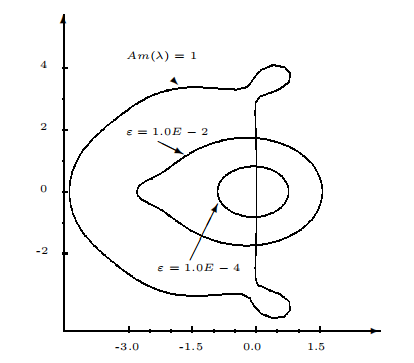
\includegraphics[width=7cm,height=7cm]{./figures/1.png}
			\caption{$EuExp_{4}^{3}$的稳定性和精度区域}
			\label{5.1}
		\end{minipage}
	}	
	{
		\begin{minipage}{6cm}
			\centering
			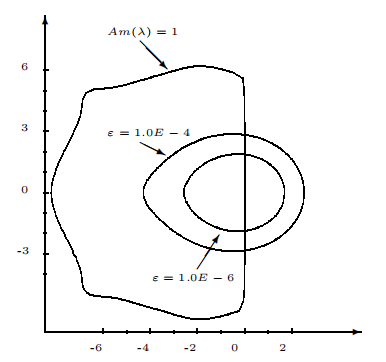
\includegraphics[width=7cm,height=7cm]{./figures/2.png}
			\caption{$EuExp_{8}^{7}$的稳定性和精度区域}
			\label{5.2}
		\end{minipage}
	}
\end{figure}
\begin{figure}[H]
	{
		\begin{minipage}{6cm}
			\centering
			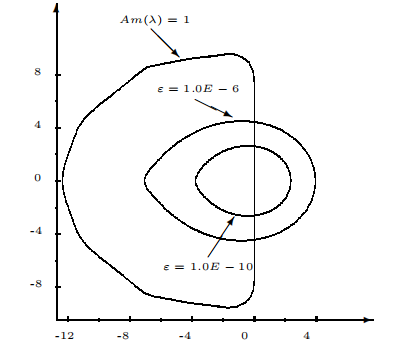
\includegraphics[width=7cm,height=7cm]{./figures/3.png}
			\caption{$EuExp_{13}^{12}$的稳定性和精度区域}
			\label{5.3}
		\end{minipage}
	}
	{
		\begin{minipage}{6cm}
			\centering
			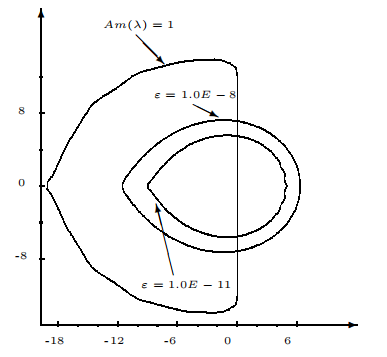
\includegraphics[width=7cm,height=7cm]{./figures/4.png}
			\caption{$EuExp_{20}^{19}$的稳定性和精度区域}
			\label{5.4}
		\end{minipage}
	}
\end{figure}

$1$.在所有情况下,稳定性条件都是由精度条件决定的。换句话说,当$Re(\lambda)<0$时,该方案达到合理的精度,方案是稳定的。\\

$2$.稳定性区域和精度区域的大小都随方案阶数的增大而增大,当$\lambda$为纯虚的情况下,$20$阶方案需要每波长约$20$个节点才能达到$11$位精度。\\

\textbf{注5.1} 显然,Euler方法并不是可以应用延迟修正方法的最有效的求解方法。例如,我们用显式Adams方法进行了实验,其阶数最多为$6$,并且在所需的函数计算次数方面得到了最多为$3$倍的改进。\\
\subsection{$EuImp$格式的稳定性和精度性}

对于多个组合$m,J$,我们数值构造了格式$EuImp^{J}_{m}$的稳定性和精度区域的边界(图\ref{5.5}-\ref{5.12})。这些格式的稳定性区域扩展到无穷大;换句话说,它们在标记为$Am(\lambda)=1$的边界之外是稳定的。值得注意的是,在大多数情况下,不稳定区域比精确区域大得多。因此,我们为每个方案提供了两个数字。第一种是相对粗糙的尺度,描述了稳定区域。第二种方法的尺度要细得多,它描述了两个选定精度的精度区域;在后一种情况下,稳定区域的边界几乎与虚轴没有区别。每个图形都带有一个图例,说明了该方案的详细稳定性特征(所有方案$EuImp^{J}_{m}$都是$A(\alpha)$-稳定的,图中指定了$\alpha$的数值近似值)。所有的$EuImp^{J}_{m}$方案都不是$L$-稳定的;图中指定了每个方案$\mu$的值(见($4.3$))。\\
\begin{figure}[htbp]
	{
		\begin{minipage}{6cm}
			\centering
			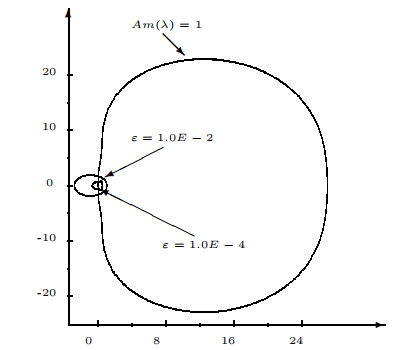
\includegraphics[width=7cm,height=7cm]{./figures/5.png}
			\caption{$EuImp_{4}^{3},\mu \approx -.3913,\alpha = 90^{\circ}$的稳定性和精度区域}
			\label{5.5}
		\end{minipage}
	}
	{
		\begin{minipage}{6cm}
			\centering
			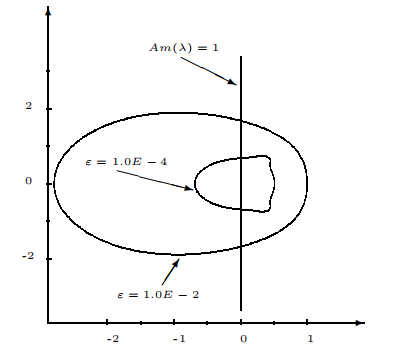
\includegraphics[width=7cm,height=7cm]{./figures/6.png}
			\caption{$EuImp_{4}^{3}$的稳定性和精度区域的详细说明}
			\label{5.6}
		\end{minipage}
	}
\end{figure}
\begin{figure}[htbp]
	{
		\begin{minipage}{6cm}
			\centering
			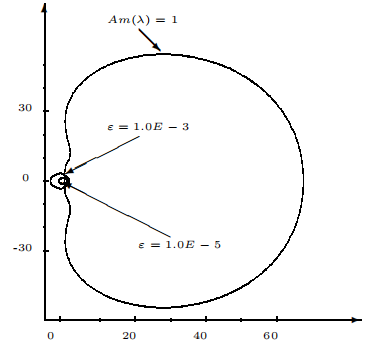
\includegraphics[width=7cm,height=7cm]{./figures/7.png}
			\caption{$EuImp_{6}^{5},\mu \approx -.3101, \alpha \approx 89.979^{\circ}$的稳定性和精度区域}
			\label{5.7}
		\end{minipage}
	}
	{
		\begin{minipage}{6cm}
			\centering
			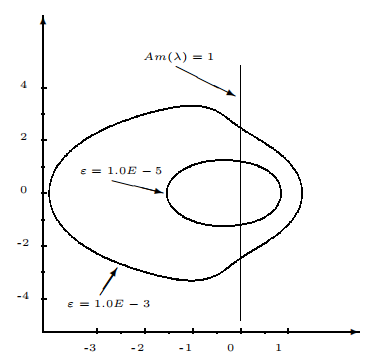
\includegraphics[width=7cm,height=7cm]{./figures/8.png}
			\caption{$EuImp_{6}^{5}$的稳定性和精度区域的详细说明}
			\label{5.8}
		\end{minipage}
	}
\end{figure}
\begin{figure}[htbp]
	{
		\begin{minipage}{6cm}
			\centering
			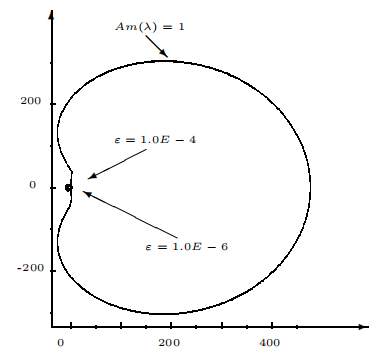
\includegraphics[width=7cm,height=7cm]{./figures/9.png}
			\caption{$EuImp_{12}^{11},\mu \approx 0.1369, \alpha \approx 76.8^{\circ}$的稳定性和精度区域}
			\label{5.9}
		\end{minipage}
	}
	{
		\begin{minipage}{6cm}
			\centering
			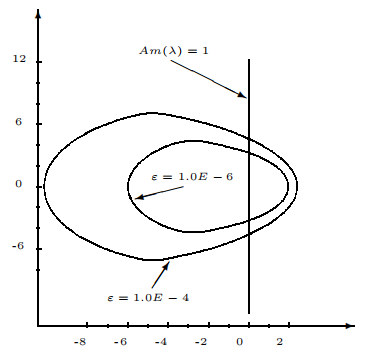
\includegraphics[width=7cm,height=7cm]{./figures/10.png}
			\caption{$EuImp_{12}^{11}$的稳定性和精度区域的详细说明}
			\label{5.10}
		\end{minipage}
	}
\end{figure}
\begin{figure}[htbp]
	{
		\begin{minipage}{6cm}
			\centering
			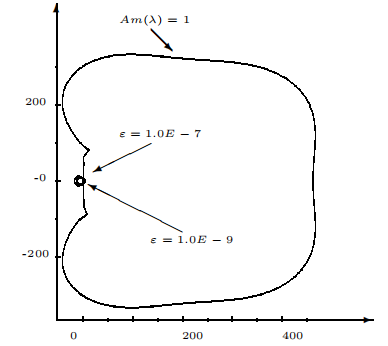
\includegraphics[width=7cm,height=7cm]{./figures/11.png}
			\caption{$EuImp_{20}^{19},\mu \approx -0.3030, \alpha \approx 77.5^{\circ}$的稳定性和精度区域}
			\label{5.11}
		\end{minipage}
	}
	{
		\begin{minipage}{6cm}
			\centering
			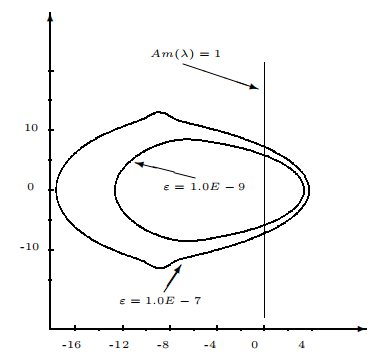
\includegraphics[width=7cm,height=7cm]{./figures/12.png}
			\caption{$EuImp_{20}^{19}$的稳定性和精度区域的详细说明}
			\label{5.12}
		\end{minipage}
	}
\end{figure}
从图\ref{5.5}-\ref{5.12}可以得出几个观察结果。\\

$1$.有一些$EuImp^{J}_{m}$方案是$A$-稳定的,最高可达$4$阶(如$EuImp^3_4$)。$EuImp^5_6$ 方案是$A(\alpha)$-稳定的,$\alpha>89.5^{\circ}$;在大多数实际应用中,这种方案可以看作是$A$-稳定的。对于较高的阶数,$EuImp^{J}_{m}$的$A$-稳定性性能迅速恶化(见图\ref{5.9}-\ref{5.12})。\\

$2$.$EuImp^{J}_{m}$中没有一个方案是$L$-稳定的。然而,在我们已经研究过的所有情况下,$\mu$小于$1/2$;虽然$L$-稳定性($\mu=0$) 是非常理想的,但$\mu<1/2$保证了在许多情况下足够的衰减速率。\\

$3$.对于实的和复的$\lambda$,我们所测试的所有方法的精度区域都是非常令人满意的。例如,从图\ref{5.8}可以很容易看出,$EuImp^5_6$(一种$6$阶方案)需要每个波长大约$18$个节点才能获得$3$位数字;该数目增加到每波长约$40$个节点才能得到$5$位数字,这表明需要更高级别的方案。这类计划将在下一小节中讨论。\\
\subsection{$EuComb$格式的稳定性和精确性}

对于$m_1,m_2,j_1,j_2$的一系列组合,我们用数值方法构造了$EuComb_{m_1,m_2}^{j_1,j_2}$格式的稳定性和精度区域的边界。与$EuComb$格式一样,这些格式的稳定性区域扩展到无穷大;它们在标有$Am(\lambda)=1$的边界之外是稳定的。对于简单的$EuImp$格式,不稳定区域一般比精度区域大得多。因此,我们再次为每种情况提供两个数字。第一种是相对粗糙的尺度,描述了稳定区域。第二种是在一个更精细的尺度上,描述了两个选定精度的精确区域;在后一种情况下,稳定区域的边界几乎与虚轴没有区别。每个图形都有一个图例,详细说明了方案的稳定性特征。所有的$EuComb^J_m$格式都是$A(\alpha)$-稳定的,图解描述了数值计算得到的$\alpha$的近似值。由于所有的格式$EuComb^J_m$都是$L$- 稳定的(见定理$4.3$),所以我们不指定每个方案的$\mu$值。\\
\begin{figure}[H]
	{
		\begin{minipage}{6cm}
			\centering
			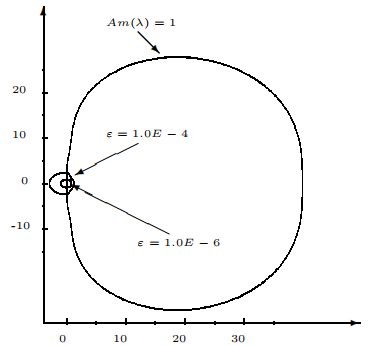
\includegraphics[width=7cm,height=7cm]{./figures/13.png}
			\caption{$EuComb_{6,5}^{5,5},\alpha = 90^{\circ}$的稳定性和精度区域}
			\label{5.13}
		\end{minipage}
	}
	{
		\begin{minipage}{6cm}
			\centering
			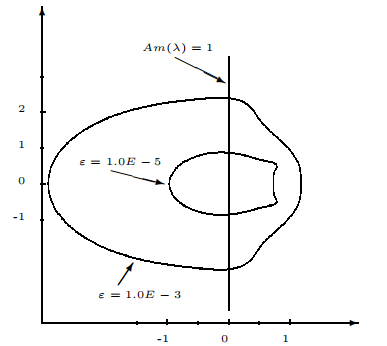
\includegraphics[width=7cm,height=7cm]{./figures/14.png}
			\caption{$EuComb_{6,5}^{5,5}$的稳定性和精度区域的详细说明}
			\label{5.14}
		\end{minipage}
	}
\end{figure}
\begin{figure}[H]
	{
		\begin{minipage}{6cm}
			\centering
			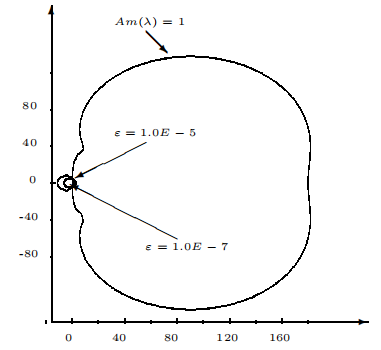
\includegraphics[width=7cm,height=7cm]{./figures/15.png}
			\caption{$EuComb_{13,12}^{12,12}, \alpha \approx 89.9914^{\circ}$的稳定性和精度区域}
			\label{5.15}
		\end{minipage}
	}
	{
		\begin{minipage}{6cm}
			\centering
			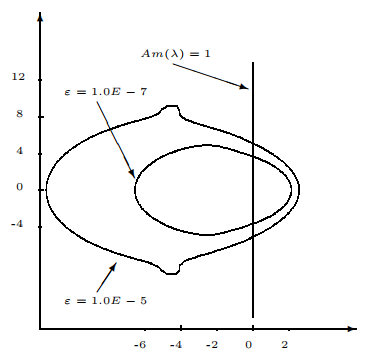
\includegraphics[width=7cm,height=7cm]{./figures/16.png}
			\caption{$EuComb_{13,12}^{12,12}$的稳定性和精度区域的详细说明}
			\label{5.16}
		\end{minipage}
	}
\end{figure}
\begin{figure}[H]
	{
		\begin{minipage}{6cm}
			\centering
			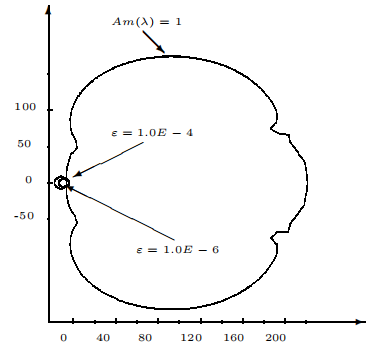
\includegraphics[width=7cm,height=7cm]{./figures/17.png}
			\caption{$EuComb_{16,15}^{15,15}, \alpha \approx 89.994^{\circ}$的稳定性和精度区域}
			\label{5.17}
		\end{minipage}
	}
	{
		\begin{minipage}{6cm}
			\centering
			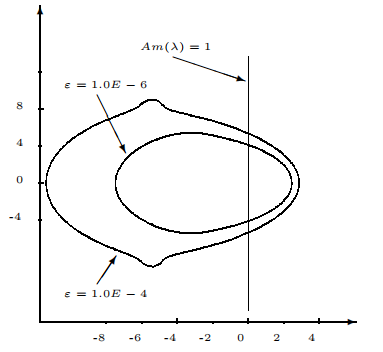
\includegraphics[width=7cm,height=7cm]{./figures/18.png}
			\caption{$EuComb_{16,15}^{15,15}$的稳定性和精度区域的详细说明}
			\label{5.18}
		\end{minipage}
	}
\end{figure}
\begin{figure}[H]
	{
		\begin{minipage}{6cm}
			\centering
			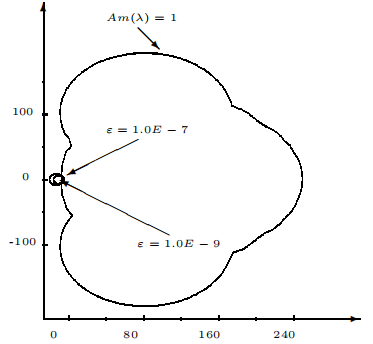
\includegraphics[width=7cm,height=7cm]{./figures/19.png}
			\caption{$EuComb_{17,16}^{16,16}, \alpha \approx 89.014^{\circ}$的稳定性和精度区域}
			\label{5.19}
		\end{minipage}
	}
	{
		\begin{minipage}{6cm}
			\centering
			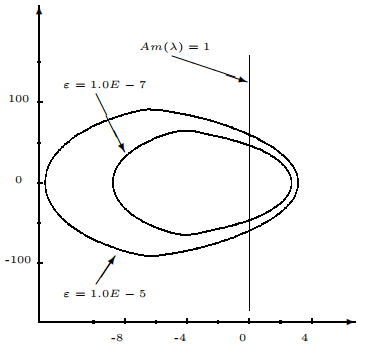
\includegraphics[width=7cm,height=7cm]{./figures/20.png}
			\caption{$EuComb_{17,16}^{16,16}$的稳定性和精度区域的详细说明}
			\label{5.20}
		\end{minipage}
	}
\end{figure}
\begin{figure}[H]
	{
		\begin{minipage}{6cm}
			\centering
			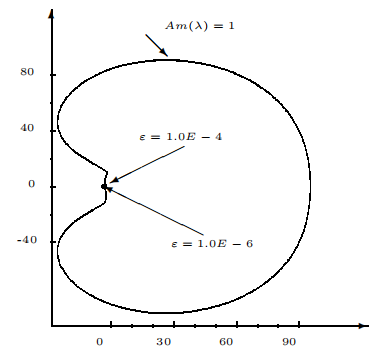
\includegraphics[width=7cm,height=7cm]{./figures/21.png}
			\caption{$EuComb_{8,6}^{6,6}, \alpha \approx 55.786^{\circ}$的稳定性和精度区域}
			\label{5.21}
		\end{minipage}
	}
	{
		\begin{minipage}{6cm}
			\centering
			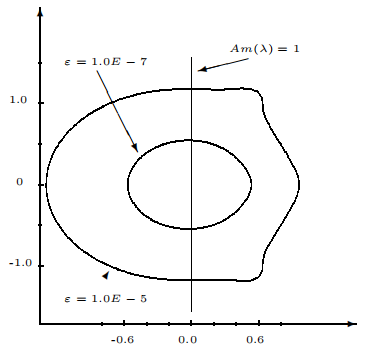
\includegraphics[width=7cm,height=7cm]{./figures/22.png}
			\caption{$EuComb_{8,6}^{6,6}$的稳定性和精度区域的详细说明}
			\label{5.22}
		\end{minipage}
	}
\end{figure}
\begin{figure}[H]
	{
		\begin{minipage}{6cm}
			\centering
			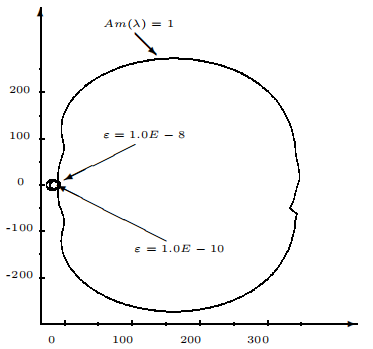
\includegraphics[width=7cm,height=7cm]{./figures/23.png}
			\caption{$EuComb_{20,19}^{19,19}, \alpha \approx 89.9969^{\circ}$的稳定性和精度区域}
			\label{5.23}
		\end{minipage}
	}
	{
		\begin{minipage}{6cm}
			\centering
			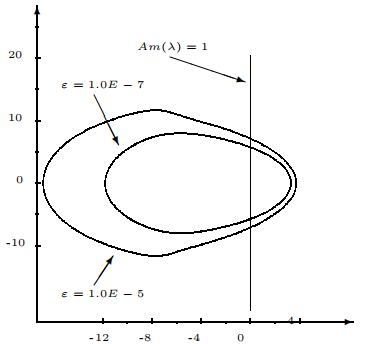
\includegraphics[width=7cm,height=7cm]{./figures/24.png}
			\caption{$EuComb_{20,19}^{19,19}$的稳定性和精度区域的详细说明}
			\label{5.24}
		\end{minipage}
	}
\end{figure}
从图\ref{5.13}-\ref{5.24}可以得出几个观察结果。\\

$1$.存在$A$-稳定的$EuImp^J_m$方案,最多可达$5$阶(例如,$EuComb^{5,5}_{6,5}$)。我们已经测试所有阶数(多达$30$阶甚至更多),存在$\alpha$非常接近$90^{\circ}$ 的$A(\alpha)$- 稳定方案。例如,$EuComb_{12,12}^{12,12}$具有$12$阶(见定理$4.1$),且是$A(\alpha)$-稳定的,$\alpha>89.99^{\circ}$。$EuComb^{19,19}_{20,19}$为$19$阶,是$A(\alpha)$-稳定的,$\alpha>89.996^{\circ}$。另一方面,在数值建立这些性质之前,我们无法可靠地预测哪些方案具有良好的稳定性,哪些方案不具有稳定性。以$EuComb^{15,15}_{16,15}$为例,$\alpha>89.99^{\circ}$,而$EuComb^{16,16}_{17,16}$,有$89.01^{\circ}<\alpha<89.02^{\circ}$。另一个极端是$EuComb^{6,6}_{8,6}$方案,其灾难性的$\alpha<56^{\circ}$(图\ref{5.21})。一般情况下,当$m_1+m_2$为偶数时,$EuComb^{j_1,j_2}_{m_1,m_2}$格式往往具有较差的稳定性。当然,这在很大程度上是一种好奇心,因为很容易获得各阶的好方案。\\

$2$.对于实的和复的$\lambda$,我们测试的所有方法的精度区域都是非常令人满意的。例如,从图\ref{5.24}可以很容易地看出,$19$阶方案$EuComb^{19,19}_{20,19}$ 每波长大约需要$18$个节点才能获得$10$位数字。\\
\section{自适应实现}

在常微分方程组数值解的实际应用中,自适应行进、精度控制等问题发挥着重要作用。由于本文的方案本质上是单步的,因此在其自适应实现中产生的大多数问题相对简单。同样值得注意的是,当底层求解器具有高收敛阶时,精度控制要简单得多。\\

我们已经实现了$EuExp,EuImp,EuComb$等方案的完全自适应版本。在本节中,我们描述了实现的一些技术细节,而下一节描述了我们所做的一些数值实验。我们将使用$EuExp$作为我们的模型来讨论这些问题;另外两个方案($EuImp$和$EuComb$)遇到相同的问题,以类似的方式处理。\\
\subsection{精度控制}

给定区间$[a,b]$上的初值问题(\ref{1.1}),(\ref{1.2}),一个近似解$EuExp^J_m(F,\varphi_a)$和一个正数$\epsilon$,我们想确定是否\\
\begin{equation}
\label{6.1}
|EuExp^J_m(F,\varphi_a)-\varphi|<\epsilon.
\end{equation}
显然,这是不完全可靠的;所有现有技术的目的都是以可接受的代价,以极高的概率作出决定。幸运的是,方法$EuExp^J_m$的内部结构为我们提供了许多可以检查的条件。从我们的经验来看,下面列出的条件是完全可靠的。\\

$1$.验证了修正过程已收敛到精度$\epsilon$。换句话说,我们要求向量$\delta$的范数(见(\ref{2.14}))在最后一次校正期间得到的范数小于$\epsilon$。这并不保证(\ref{6.1});它确实表明校正方案在内部与精度$\epsilon$一致。\\

$2$.在区间$[a,b]$的高斯节点上得到了$EuExp^J_m(F,\varphi_a)$的近似解。我们将算子$W^m$应用于$EuExp^J_m(F,\varphi_a)$,得到了它的勒让德展开的$m$个系数(见(\ref{2.26})。如果$EuExp^J_m(F,\varphi_a)$的离散化足够精细,则勒让德展开的最后几个系数必须很小。在我们的实现中,我们要求后两个系数小于$\epsilon$。\\

$3$.另一次测试我们尝试同时验证校正过程和离散化是否收敛到精度$\epsilon$。当对$EuExp^J_m(F,\varphi_a)$进行求值后,通过插值求出$b$点的近似解的值(见注$4.1$),并将插值过程应用于$EuExp^J_m(F,\varphi_a)$和$EuExp^{J-1}_m(F,\varphi_a)$,并要求差值小于$\epsilon$。\\

$4$.在极端情况下,ODE的解可能解得很差而变得不稳定;通常的结果是指数溢出。为了防范这种情况,我们在欧拉过程的每一步都检查解的大小;如果该解足够大(我们任意将阈值设置为$10^{35}$),则认为问题未得到解决。\\
\subsection{步长控制}

我们在这里的方法是完全标准的。我们从或多或少的任意步长开始,并尝试应用$EuExp^J_m$方案。如果结果的精度不够(根据上面$(1)-(4)$的标准),则步长减半,并重复该过程。如果精度令人满意,则步长不变。如果精度连续两步令人满意,则步长增加一倍。\\
\subsection{线性隐式实现}

为了减少函数求值的次数,在大多数外推代码中,一个常见的做法是使用行进方案$[11]$的“线性隐式”公式。对于常微分方程\\
\begin{equation}
\varphi'(t)=F(t,\varphi(t)),~~~~~~t \in [a,b]
\label{6.2}
\end{equation}
在近似解$\varphi_0(t)$的情况下,我们让$\varphi=\varphi_0+\delta$,(\ref{6.2})写成\\
$$\varphi'_0(t)+\delta'(t)=F(t,\varphi_0(t)+\delta(t))$$
或\\
\begin{equation}
\delta(t)=\int_a^t F(\tau,\varphi_0(\tau)+\delta(\tau))~d\tau-\varphi_0(t).
\label{6.3}
\end{equation}
但对于小$\delta$\\
$$F(t,\varphi_0(t)+\delta(t))=F(t,\varphi_0(t))+J_{\varphi_0}(t) \delta(t)+O(\| \delta \|^2)$$
其中$J_{\varphi_0}(t)$表示$F$在点$(t,\varphi_0(t)$的雅克比矩阵的第二个参数。代入(\ref{6.3})得\\
\begin{equation}
\label{6.4}
\delta(t)=\int_a^t J_{\varphi_0}(t)\delta(\tau)~d\tau+ \int_a^t F(\tau,\varphi_0(\tau))~d\tau-\varphi_0(t)
\end{equation}
然后,我们可以使用向后欧拉方法应用于(\ref{6.4})的延迟校正过程。我们的线性隐式代码对这个方程执行最多六步延迟修正,然后根据以下内容更新近似解$\varphi_0$\\
$$\varphi_0(t) := \varphi_0(t)+\delta(t)$$
\section{数值实验}

通过两个例子说明了谱延迟校正方法的性能。首先是由雅可比椭圆函数$sn,cn,dn$满足的三个常微分方程组\\
$$ sn'(t)=cn(t) \cdot dn(t),$$
$$cn'(t)=-sn(t) \cdot dn(t),$$
$$dn'(t)= -\mu \cdot sn(t) \cdot cn(t),$$
在$\mu=0.5$,初始数据为$sn(0)=0,cn(0)=1,dn(0)=1$的区间$[0,1]$上,这是非刚性问题的常见模型。从图\ref{7.1}的结果可以看出,为了获得最优的性能,该方法的精度阶数应该随着期望精度的增加而增加。\\
\begin{figure}[h]
	\centering
	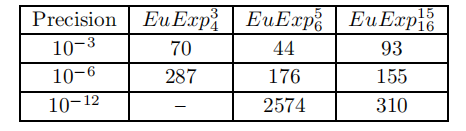
\includegraphics[width=10cm,height=3cm]{./figures/71.png}
	\caption{我们第一个(非刚性)例子的低、中、高阶谱延迟校正方法的性能。第一列表示要求的精度,其余列列出相应方案所需的函数调用数。}
	\label{7.1}
\end{figure}
我们的第二个例子是$Van der Pol$振子,这是一个著名的由两个方程组成的刚性系统\\
$$y'_1(t)=y_2(t)$$
$$y'_2(t)=(1-y_1^2(t)y_2(t))/ \epsilon -y_1(t),$$
其中$y_1(0)=2,y_2(0)=0$。我们选择$\epsilon=10^{-6}$并在$[0,1]$区间上求解。为了便于比较,我们测试了我们的代码与这个问题上表现最好的代码之一高阶外推码$EULSIM[4]$。 结果见图\ref{72}-\ref{74}。\\
\begin{figure}[h]
	\centering
	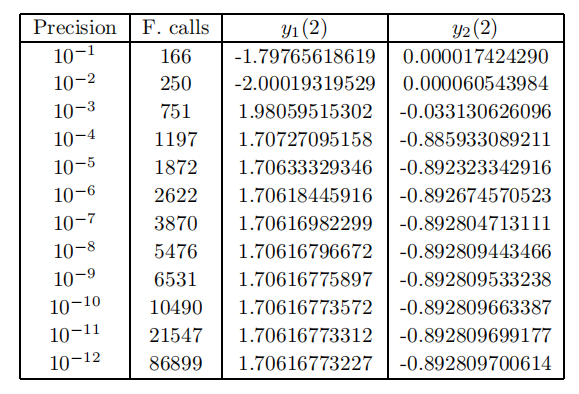
\includegraphics[width=10cm,height=6cm]{./figures/72.png}
	\caption{外推码$EULSIM$在$Van der Pol$振荡器问题上的性能。第一列表示要求的精度,第二列表示函数计算的次数,第三列列出计算出解的分量$y_1(2)$,第四列列出计算出解的分量$y_2(2)$。}
	\label{72}
\end{figure}
\begin{figure}[h]
	\centering
	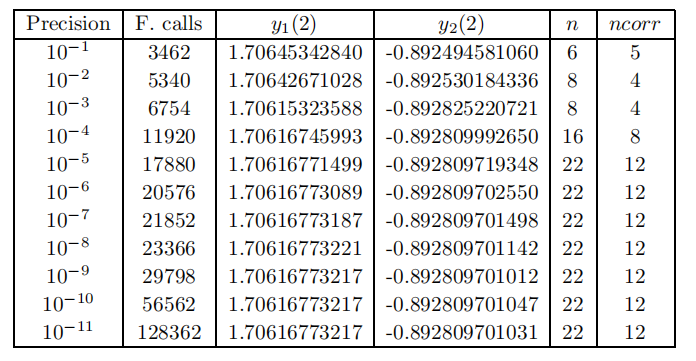
\includegraphics[width=10cm,height=5cm]{./figures/73.png}
	\caption{谱延迟校正码$EuImp$在$Van der Pol$振荡器问题上的性能。前四列对应于图\ref{72}中的列。后两列表示每个子区间上使用的点数$n$(精度的最高阶数)和代码实际使用的最大校正数$ncorr$。}
	\label{73}
\end{figure}
\begin{figure}[h]
	\centering
	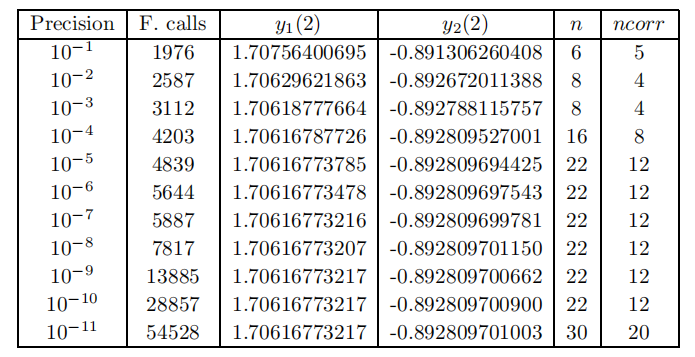
\includegraphics[width=10cm,height=5cm]{./figures/74.png}
	\caption{线性隐式谱延迟校正码在$Van der Pol$振子问题上的性能。这些列对应于图\ref{73}中的列。}
	\label{74}
\end{figure}
从这些图中可以得出一些观察结果。\\

$1$.在任何要求的精度下,$EULSIM$代码所需的函数计算明显少于$EuImp$方案。与线性隐式延迟校正代码相比,$EULSIM$还需要更少的函数计算。\\

$2$.如果比较实际的精确度,而不是要求的精确度,就会出现稍微不同的情况。该单隐延迟校正方案在请求的误差为$10^{-5}$时,使用$4839$个函数调用,实现了大约8位精度。另一方面,$EULSIM$使用$10490$个函数调用,在请求的公差为$10^{-10}$的情况下,实现了八位数的精度。这并不是为了贬低$EULSIM$的性能。\\


\section{结论}

我们认为,基于常微分方程积分方程公式的延迟修正方法是值得进一步研究的方法。它们具有优良的稳定性,易于实现,并且只需要一个好的低阶求解器来驱动过程。我们的初步实验,使用一个原始的自适应实现,与先进的外推法代码相比,具有中等到高精度。\\




\cite{tam19912d}
\bibliography{../../ref}
\end{document}













